\let\lesson\undefined
\newcommand{\lesson}{\phantomlesson{Bài 6: Định luật Boyle. Định luật Charles}}
\chapter[Định luật Charles]{Định luật Charles}
\section{Lý thuyết}
Khi áp suất của một khối lượng khí xác định được giữ không đổi thì thể tích của khí tỉ lệ thuận với nhiệt độ tuyệt đối của nó:
\begin{equation}
	\dfrac{V}{T}=\text{hằng số}\quad \text{hay} \quad \dfrac{V_1}{T_1}=\dfrac{V_2}{T_2}
\end{equation}
\begin{minipage}[t]{.45\linewidth}
	\begin{center}
		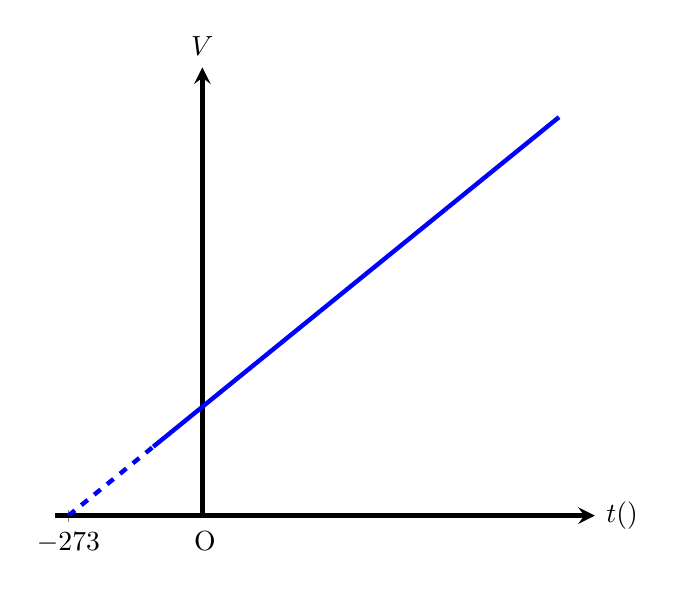
\begin{tikzpicture}  
			\begin{axis}[  ultra thick,
				xmin=-300,  
				xmax=800,  
				xtick={-273,0},
				ytick=\empty,
				ymin=0,  
				ymax=900, 
				samples=300,
				%				xticklabels=\empty,
				yticklabels=\empty,
				axis lines=center, 
				xlabel=$\xsi{t}{(\celsius)}$, 
				ylabel=$V$, 
				every axis y label/.style={at=(current axis.above origin),anchor=south},  
				every axis x label/.style={at=(current axis.right of origin),anchor=west},  ]
				\addplot [ultra thick, blue, smooth,dashed, domain=-273:-100] {0.8*(x+273)}; 
				\addplot [ultra thick, blue, smooth, domain=-100:727] {0.8*(x+273)}; 
			\end{axis}  
			\node[label={[below]90:O}] at (1.9,-0.2){};
		\end{tikzpicture}
		\captionof{figure}{Đồ thị biểu diễn sự thay đổi thể tích khí theo nhiệt độ Celsius.}
	\end{center}
\end{minipage}\hfill
\begin{minipage}[t]{.45\linewidth}
	\begin{center}
		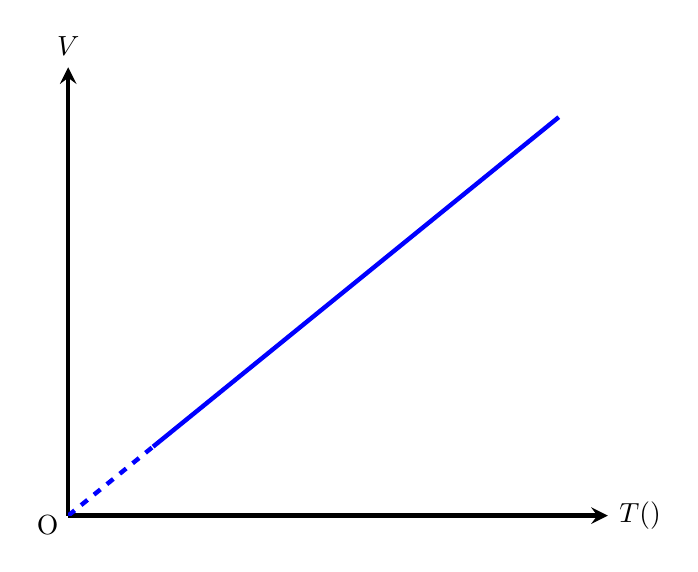
\begin{tikzpicture}  
			\begin{axis}[  ultra thick,
				xmin=0,  
				xmax=1100,  
				xtick=\empty,
				ytick=\empty,
				ymin=0,  
				ymax=900, 
				samples=300,
				xticklabels=\empty,
				yticklabels=\empty,
				axis lines=center, 
				xlabel=$\xsi{T}{(\kelvin)}$, 
				ylabel=$V$, 
				every axis y label/.style={at=(current axis.above origin),anchor=south},  
				every axis x label/.style={at=(current axis.right of origin),anchor=west},  ]
				\addplot [ultra thick, blue, smooth,dashed, domain=0:173] {0.8*x}; 
				\addplot [ultra thick, blue, smooth, domain=173:1000] {0.8*x}; 
			\end{axis}  
			\node[label={[below left]90:O}] at (0,0){};
		\end{tikzpicture}
		\captionof{figure}{Đồ thị biểu diễn sự thay đổi thể tích khí theo nhiệt độ Kelvin.}
	\end{center}
\end{minipage}
\begin{center}
	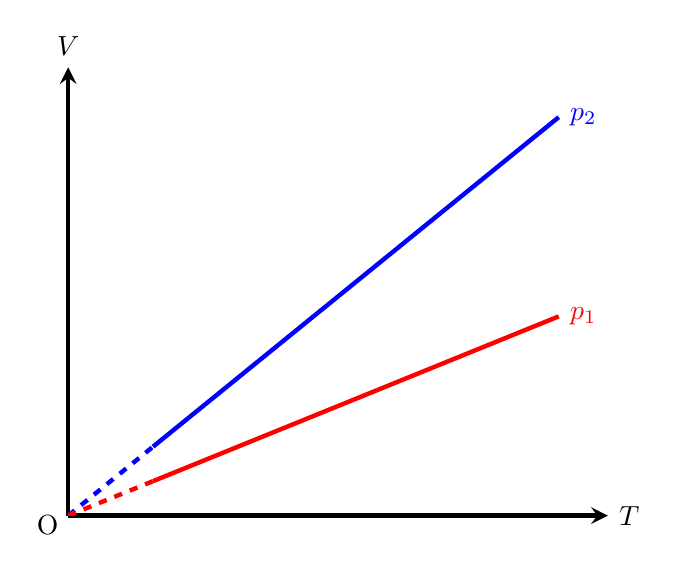
\begin{tikzpicture}  
		\begin{axis}[  ultra thick,
			xmin=0,  
			xmax=1100,  
			xtick=\empty,
			ytick=\empty,
			ymin=0,  
			ymax=900, 
			samples=300,
			xticklabels=\empty,
			yticklabels=\empty,
			axis lines=center, 
			xlabel=$T$, 
			ylabel=$V$, 
			every axis y label/.style={at=(current axis.above origin),anchor=south},  
			every axis x label/.style={at=(current axis.right of origin),anchor=west},  ]
			\addplot [ultra thick, blue, smooth,dashed, domain=0:173] {0.8*x}; 
			\addplot [ultra thick, blue, smooth, domain=173:1000] {0.8*x} node[right]{$p_2$}; 
			\addplot [ultra thick, red, smooth,dashed, domain=0:173] {0.4*x}; 
			\addplot [ultra thick, red, smooth, domain=173:1000] {0.4*x} node[right]{$p_1$};
		\end{axis}  
		\node[label={[below left]90:O}] at (0,0){};
	\end{tikzpicture}
	\captionof{figure}{Các đường đẳng áp của một khối khí lí tưởng ứng với các áp suất $p_1$ và $p_2 \left(p_2<p_1\right)$.}
\end{center}
\luuy{Định luật Boyle và định luật Charles là các định luật đúng với khí lí tưởng, gần đúng với khí thực. Trong điều kiện áp suất cao và nhiệt độ thấp, kết quả thực nghiệm khí thực không phù hợp với các định luật trên.}
\section{Mục tiêu bài học - Ví dụ minh hoạ}
\begin{dang}{Vận dụng được định luật Charles}
	\viduii{2}
	{Cho một khối khí dãn nở đẳng áp từ nhiệt độ $t_1=\SI{32}{\celsius}$ đến nhiệt độ $t_2=\SI{117}{\celsius}$, thể tích khối khí tăng thêm 1,7 lít. Xác định thể tích khối khí trước và sau khi dãn nở.
	
}
{\hide{
	\begin{center}
		\begin{tabular}{C{4cm} C{1.5cm} C{4.5cm}}
			\colorbox{yellow}{\textcolor{red}{\textbf{Trạng thái 1}}} & $\xrightarrow[]{p=const}$ & \colorbox{yellow}{\textcolor{red}{\textbf{Trạng thái 2}}}\\
			$T_1=\SI{305}{\kelvin}$ & &$T_2=\SI{390}{\kelvin}$\\
			$V_1=?$ & & $V_2=V_1+\SI{1.7}{\text{lít}}$
		\end{tabular}
	\end{center}
Theo định luật Charles:
\begin{eqnarray*}
	&&\dfrac{V_1}{T_1}=\dfrac{V_2}{T_2}\\
	&\Leftrightarrow& \dfrac{V_1}{\SI{305}{\kelvin}}=\dfrac{V_1+\SI{1.7}{\text{lít}}}{\SI{390}{\kelvin}}\\
	&\Rightarrow& V_1=\SI{6.1}{\text{lít}}.
\end{eqnarray*}
}}

\viduii{3}
{Một mô hình áp kế gồm một bình cầu thuỷ tinh có thể tích $\SI{270}{\centi\meter^3}$ gắn với một ống nhỏ nằm ngang có tiết diện $\SI{0.1}{\centi\meter^2}$. Trong ống có một giọt thuỷ ngân. Ở $\SI{0}{\celsius}$ giọt thuỷ ngân cách miệng bình cầu $\SI{30}{\centi\meter}$. Tính khoảng di chuyển của giọt thuỷ ngân khi hơ nóng bình cầu đến $\SI{10}{\celsius}$. Coi thể tích bình là không đổi và ống thuỷ tinh đủ dài để giọt thuỷ ngân không rơi ra ngoài.
\begin{center}
	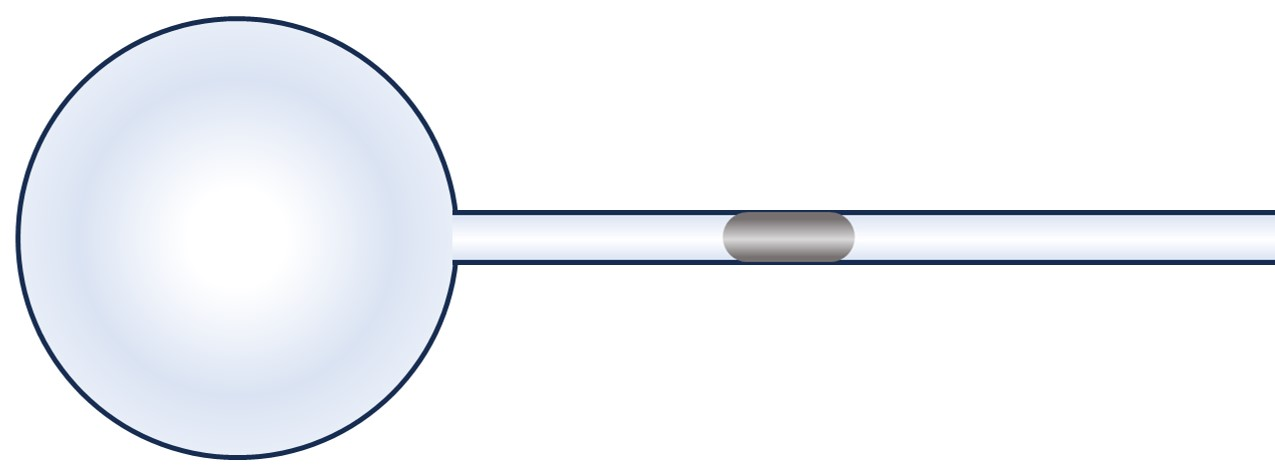
\includegraphics[width=0.35\linewidth]{../figs/VN12-Y24-PH-SYL-011-1}
\end{center}
}
{\hide{
	Gọi:
	\begin{itemize}
		\item $S$ là tiết diện ống thuỷ tinh, $S=\SI{0.1}{\centi\meter^2}$;
		\item $V$ là thể tích bình cầu;
		\item $\ell_1$, $\ell_2$ lần lượt là khoảng cách từ giọt thuỷ ngân đến miệng bình trước và sau khi hơ nóng.
	\end{itemize} 
Giọt thuỷ ngân cân bằng khi áp suất khí trong bình cân bằng với áp suất khí ngoài bình. Do đó, quá trình hơ nóng bình xem như quá trình biến đổi trạng thái đẳng áp của khí trong bình.
\begin{center}
	\begin{tabular}{C{4cm} C{1.5cm} C{5cm}}
		\colorbox{yellow}{\textcolor{red}{\textbf{Trạng thái 1}}} & $\xrightarrow[]{p=const}$ & \colorbox{yellow}{\textcolor{red}{\textbf{Trạng thái 2}}}\\
		$T_1=\SI{273}{\kelvin}$ & &$T_2=\SI{283}{\kelvin}$\\
		$V_1=V+\ell_1S=\SI{273}{\centi\meter^3}$ & & $V_2=V+\ell_2S=\xsi{\left(270+0,1\ell_2\right)}{\centi\meter^3} $
	\end{tabular}
\end{center}
Theo định luật Charles:
\begin{eqnarray*}
	&&\dfrac{V_1}{T_1}=\dfrac{V_2}{T_2}\\
	&\Leftrightarrow& \dfrac{\SI{273}{\centi\meter^3}}{\SI{273}{\kelvin}}=\dfrac{\xsi{\left(270+0,1\ell_2\right)}{\centi\meter^3}}{\SI{283}{\kelvin}}\\
	&\Rightarrow& \ell_2=\SI{130}{\centi\meter}
\end{eqnarray*}
Vậy: giọt thuỷ ngân đã di chuyển 1 đoạn $\Delta \ell=\ell_2-\ell_1=\SI{100}{\centi\meter}$.
}}
	
\end{dang}

	
